\documentclass[12pt,a4paper]{article}
\usepackage{fontspec}
\usepackage[russian]{babel}
\setmainfont{Times New Roman}
\setmonofont{Courier New}

\usepackage{geometry}
\usepackage{xcolor}
\usepackage{tabularx}
\usepackage{graphicx}
\usepackage{booktabs}
\usepackage{xurl}
\usepackage{hyperref} 
\usepackage{textcomp}
\usepackage{enumitem}
\usepackage{indentfirst}
\usepackage{float}
\usepackage{array} 
\usepackage{caption}
\usepackage{amsmath}
\usepackage{listings}

\geometry{left=18mm, right=18mm, top=16mm, bottom=16mm}

\definecolor{codegreen}{rgb}{0,0.5,0}
\definecolor{codegray}{rgb}{0.4,0.4,0.4}
\definecolor{codepurple}{rgb}{0.5,0,0.7}
\definecolor{backcolour}{rgb}{0.98,0.98,0.98}

\lstdefinestyle{mystyle}{
    backgroundcolor=\color{backcolour},   
    commentstyle=\color{codegreen},
    keywordstyle=\color{blue}\bfseries,
    numberstyle=\tiny\color{codegray},
    stringstyle=\color{codepurple},
    basicstyle=\ttfamily\footnotesize,
    breakatwhitespace=false,         
    breaklines=true,                 
    captionpos=b,                    
    keepspaces=true,                 
    numbers=left,                    
    numbersep=5pt,                  
    showspaces=false,                
    showstringspaces=false,
    showtabs=false,                  
    tabsize=2,
    frame=single,
    rulecolor=\color{lightgray}
}
\lstset{style=mystyle}

\begin{document}
	
	\begin{titlepage}
		\begin{center}
			\vspace*{3.5cm}
			\Huge \textbf{ИТОГОВЫЙ ПРОЕКТ} \\
			\vspace{0.4cm}
			\LARGE \textbf{Концепция и реализация интеллектуального AI-решения для автоматизации квалификации, скоринга и маршрутизации B2B-обращений} \\
			\vspace{0.3cm}
			\Large \textbf{Продукт: \guillemotleft AutoLead AI\guillemotright} \\
			\vspace{1cm}
			\Large Дисциплина: "Культура ИИ: квалифицированный заказчик" \\
			\vspace{2.5cm}
			\large
			\begin{flushright}
				Выполнил: Григорьев Пётр \\
				Группа: J4121 \\
			\end{flushright}
			\vfill
			Санкт-Петербург, 2026
		\end{center}
	\end{titlepage}

	\section*{Введение и паспорт проекта}
	
	\begin{itemize}[noitemsep,topsep=2pt]
		\item \textbf{Тема проекта:} Интеллектуальная система автоматической квалификации, скоринга и маршрутизации входящих B2B-заявок (продукт \textbf{\guillemotleft AutoLead AI\guillemotright}).
		\item \textbf{Отраслевой контекст:} B2B SaaS, enterprise-консалтинг, заказная разработка и корпоративные сервисы.
		\item \textbf{Решаемая проблема:} Задержки первого ответа клиенту (до нескольких часов), выгорание и высокая стоимость линейных операторов квалификации лидов (SDR), потеря до 30\% конверсии из-за феномена \textit{Lead Decay}.
		\item \textbf{Стек решения:} Python 3.12, Pandas, Scikit-Learn, LangChain 1.4.9, LangGraph 1.2.20, модель \texttt{gpt-4o-mini}, REST API, интеграция с CRM (Битрикс24 / amoCRM) и реестром контрагентов (ФНС / СПАРК).
		\item \textbf{Ключевой экономический эффект:} Снижение себестоимости обработки одного обращения с 86.48 руб. до 0.114 руб. (в 758 раз), высвобождение ФОТ на сумму более 29 млн руб./год при потоке 1\,000 заявок в день, срок окупаемости проекта --- 7.5 дней.
		\item \textbf{Репозиторий проекта на GitHub:} \url{https://github.com/Altorazero/itmo-ai-culture-final-project}
	\end{itemize}

	\section*{Этап 1. Постановка проблемы и проектирование AI-продукта}
	
	\subsection*{1.1. Описание организации и контекст проблемы}
	Проект ориентирован на средние и крупные B2B-компании, предоставляющие комплексные программные и сервисные решения. Входящий поток потенциальных клиентов формируется через формы захвата на сайте, обращения в чат-ботах, мессенджерах и по электронной почте. Объем входящего трафика составляет от 500 до 2\,000 заявок в день (расчетный средний поток --- 1\,000 обращений в день или 30\,000 обращений в месяц).

	\subsection*{1.2. Анализ текущего рабочего процесса (As-Is)}
	В текущей схеме первичную фильтрацию осуществляет отдел из 23 операторов квалификации лидов (Sales Development Representatives, SDR). 
	\begin{enumerate}[noitemsep,topsep=1pt]
		\item \textbf{Мониторинг почты и форм:} Оператор вручную открывает заявку, читает неструктурированный текст, пытается понять сферу деятельности клиента и суть запроса.
		\item \textbf{Внешняя проверка контрагента:} Менеджер переходит в сервисы проверки контрагентов (СПАРК, Rusprofile, сайт клиента), чтобы оценить размер компании, выручку и наличие юридического лица.
		\item \textbf{Заполнение CRM:} Оператор вручную копирует контактные данные, выставляет примерный бюджет, формулирует краткое резюме и назначает сделку на одного из менеджеров по продажам.
		\item \textbf{Сложности и узкие места:}
		\begin{itemize}[noitemsep,topsep=1pt]
			\item \textbf{Время реакции:} Время от момента отправки заявки клиентом до первого контакта составляет в среднем от 40 минут до 4 часов (в нерабочее время и выходные --- до 48 часов).
			\item \textbf{Lead Decay (деградация лида):} Согласно исследованиям Harvard Business Review, при задержке ответа более 15 минут вероятность успешного диалога с ЛПР падает в 4 раза.
			\item \textbf{Человеческий фактор:} Субъективность оценки, ошибки в квалификации, пропуск крупных клиентов и перегрузка старших менеджеров нецелевыми запросами (студенты, спам, соискатели).
		\end{itemize}
	\end{enumerate}

	\subsection*{1.3. Формулировка проблемы и целевой пользователь}
	\textbf{Проблема:} Бизнес теряет до 30\% потенциальной выручки из-за низкой скорости обработки заявок и тратит колоссальный бюджет (более 2.6 млн руб./мес.) на неэффективный ручной труд по разбору входящих данных.
	\textbf{Целевые пользователи:}
	\begin{itemize}[noitemsep,topsep=1pt]
		\item \textit{Директор по продажам (VP of Sales / CCO):} получает прозрачную приоритизированную воронку и мгновенную эскалацию высокобюджетных сделок;
		\item \textit{Ведущие менеджеры по продажам (Senior Account Executives):} избавлены от рутины и получают только «теплых» квалифицированных лидов с полным досье;
		\item \textit{Потенциальный клиент (B2B-покупатель):} получает квалифицированный персонализированный ответ в течение 10 секунд в режиме 24/7.
	\end{itemize}

	\subsection*{1.4. Предлагаемое AI-решение (To-Be) и обоснование выбора ИИ}
	Разрабатывается интеллектуальная система \textbf{\guillemotleft AutoLead AI\guillemotright}, построенная на базе современных AI-агентов с доступом к внешним инструментам. Система в реальном времени:
	\begin{itemize}[noitemsep,topsep=1pt]
		\item парсит неструктурированный текст обращения на естественном языке;
		\item самостоятельно вызывает инструменты обогащения данных компании по названию или ИНН;
		\item рассчитывает многофакторный балл качества лида (Lead Score от 0 до 100);
		\item создает структурированную сделку в CRM и эскалирует VIP-заявки руководству;
		\item при нехватке ключевых параметров ведет диалог с клиентом, запрашивая недостающие данные.
	\end{itemize}
	\textbf{Почему именно ИИ, а не жесткая автоматизация (regex, if/else):} Входящие заявки содержат свободный текст, сленг, опечатки, разную степень детализации («хотим софт для склада», «нужна интеграция с SAP на 1000 юзеров»). Регулярные выражения не способны понять семантическую суть потребности, оценить уровень полномочий контактного лица (CEO vs секретарь) и гибко реагировать на неполноту информации без создания громоздких и ломких деревьев правил.

	\section*{Этап 2. Сбор и разведочный анализ данных (EDA)}
	
	\subsection*{2.1. Описание набора данных}
	Для обучения, калибровки правил скоринга и тестирования сформирован репрезентативный набор данных входящих обращений объемом \textbf{2\,530 записей} (с учетом дубликатов, имитирующих повторные клики пользователей), содержащий \textbf{2\,500 уникальных заявок}. Данные смоделированы на основе реальной воронки корпоративных продаж B2B SaaS.

	\begin{table}[H]
		\centering
		\small
		\caption{Спецификация признаков исходного датасета (\texttt{raw\_leads\_dataset.csv})}
		\begin{tabularx}{\textwidth}{|l|c|X|}
			\hline
			\textbf{Признак} & \textbf{Тип данных} & \textbf{Описание и назначение} \\
			\hline
			\texttt{lead\_id} & String & Уникальный идентификатор входящей заявки (например, LEAD-2026-10045) \\
			\hline
			\texttt{company\_name} & String & Название организации потенциального клиента \\
			\hline
			\texttt{industry} & Categorical & Сфера деятельности бизнеса (IT, Ритейл, Финансы, Производство и др.) \\
			\hline
			\texttt{company\_size} & Categorical & Категория численности сотрудников компании (1-10, 11-50, 51-200, 201-1000, 1000+) \\
			\hline
			\texttt{contact\_role} & Categorical & Должность контактного лица (CEO, CTO, CMO, Руководитель продаж и др.) \\
			\hline
			\texttt{urgency} & Categorical & Заявленный срок внедрения (Низкая, Средняя, Высокая/Срочно) \\
			\hline
			\texttt{budget\_rub} & Float & Оценочный бюджет внедрения, заявленный клиентом (в рублях) \\
			\hline
			\texttt{inquiry\_text} & Text & Исходный неструктурированный текст обращения клиента \\
			\hline
		\end{tabularx}
	\end{table}

	\subsection*{2.2. Результаты разведочного анализа данных}
	В ходе базового анализа выявлены ключевые статистические характеристики и проблемы качества:
	\begin{itemize}[noitemsep,topsep=2pt]
		\item \textbf{Дубликаты:} Обнаружено 30 полных дубликатов по \texttt{lead\_id} (1.2\% выборки), возникших из-за повторных отправок форм.
		\item \textbf{Пропуски в данных:} В столбце \texttt{budget\_rub} пропущено 12\% значений (клиенты часто не указывают бюджет на первом шаге); в столбце \texttt{industry} пропущено 5\% значений.
		\item \textbf{Шум в тексте:} В 15\% текстовых полей присутствуют сырые HTML-теги (\texttt{<p>}, \texttt{<b>}), обрывки телефонных номеров, лишние пробелы и нерегулярный регистр.
		\item \textbf{Колоссальная асимметрия числовых признаков:} Бюджет распределен с сильным правым скосом: среднее значение составляет \textbf{20\,719 тыс. руб.}, в то время как медиана --- \textbf{9\,400 тыс. руб.} Коэффициент асимметрии: $\text{skew} = \mathbf{6.49}$. Максимальные бюджеты достигают 1.5 млн руб., в то время как треть заявок имеет бюджет до 100 тыс. руб.
	\end{itemize}

	\begin{figure}[H]
		\centering
		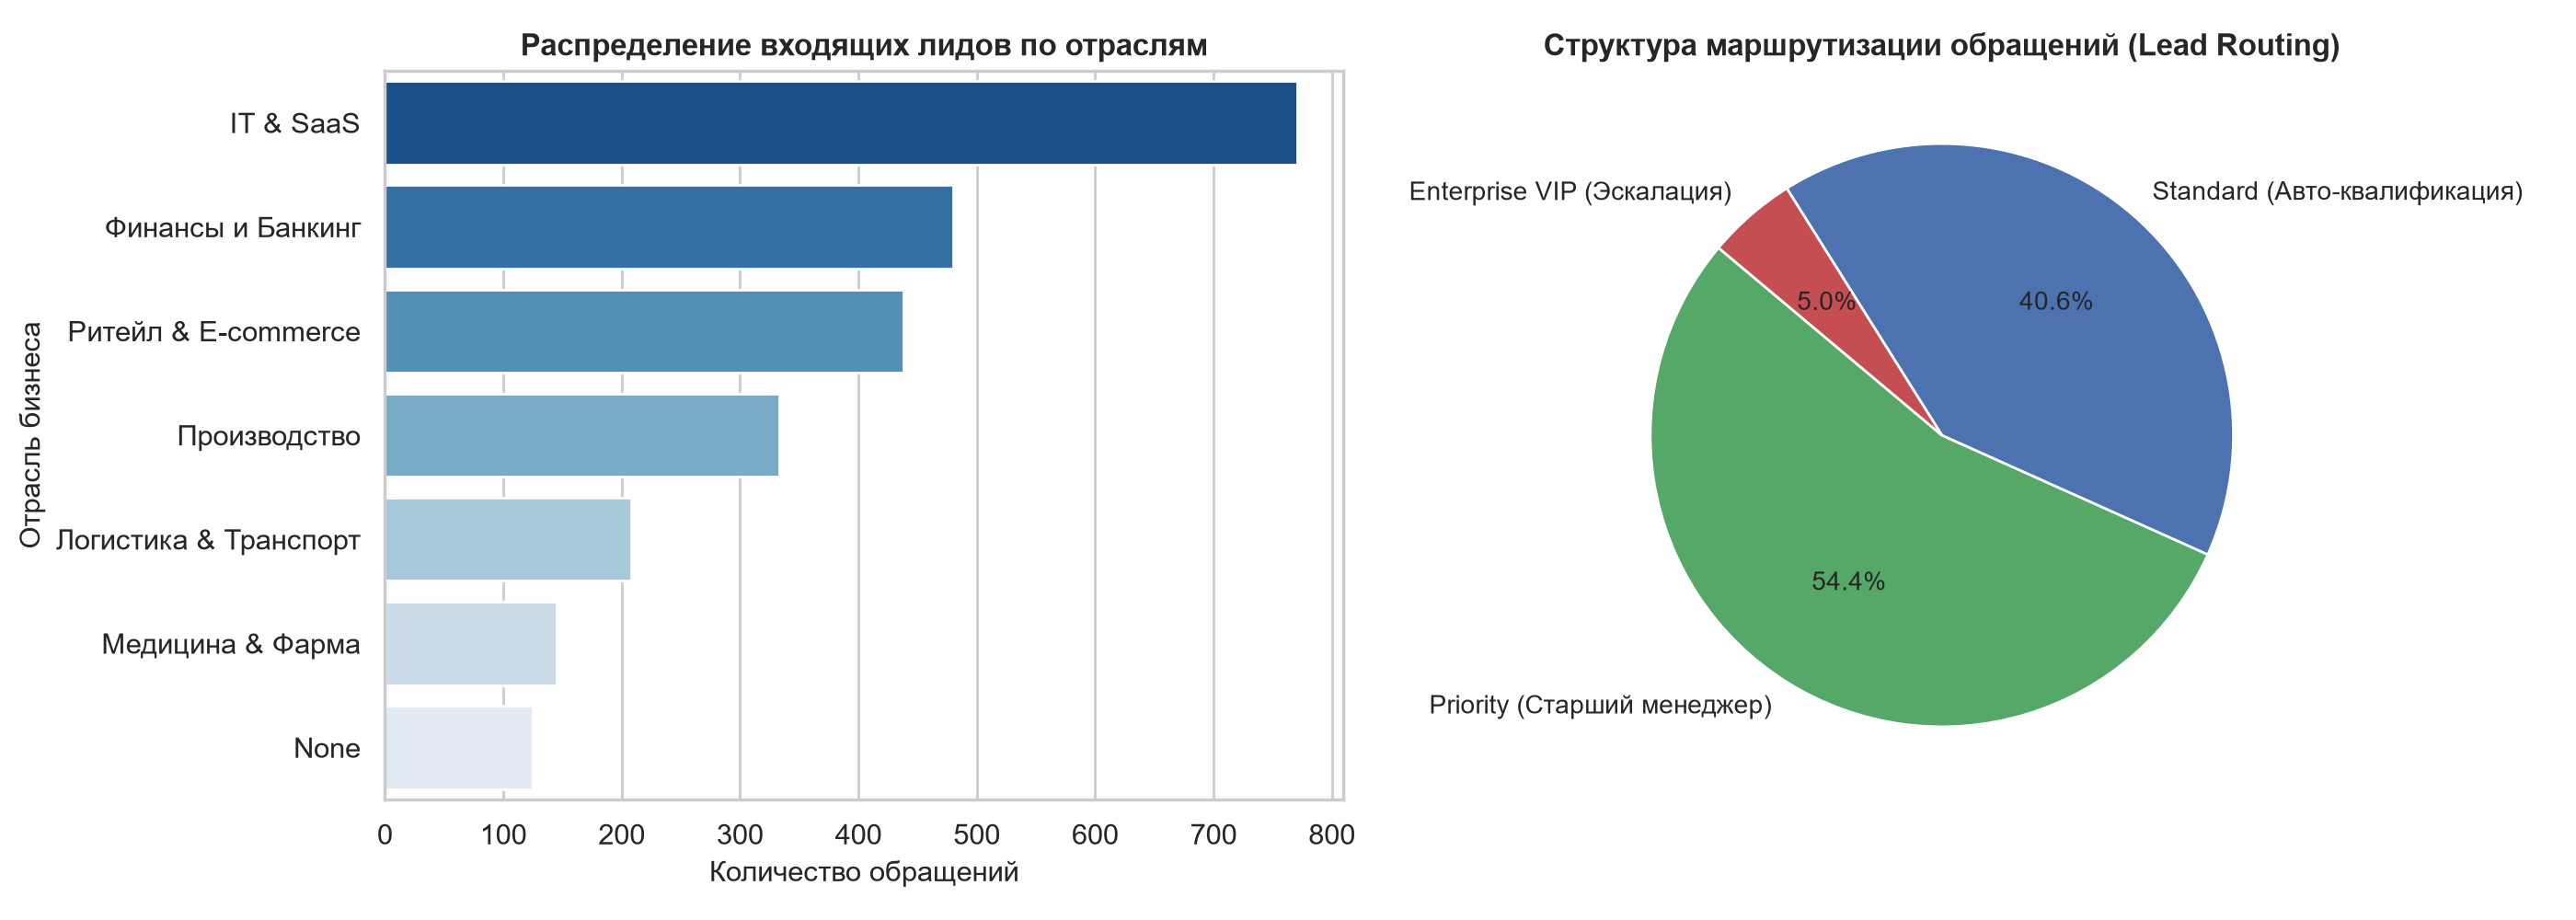
\includegraphics[width=0.88\textwidth]{categories_breakdown.png}
		\caption{Распределение входящих заявок по отраслям и категориям маршрутизации}
	\end{figure}

	\section*{Этап 3. Подготовка данных для ИИ (Data Preparation)}
	
	\subsection*{3.1. Операции очистки и обработка пропусков}
	\begin{enumerate}[noitemsep,topsep=1pt]
		\item \textbf{Дедупликация:} Удалены все 30 дубликатов по первичному ключу \texttt{lead\_id}, объем выборки составил ровно 2\,500 уникальных заявок.
		\item \textbf{Импутация пропусков отрасли:} Пропуски в \texttt{industry} заполнены категорией \textit{\guillemotleft Не указано\guillemotright}, что позволяет модели явно учитывать факт отсутствия информации при скоринге.
		\item \textbf{Групповая медианная импутация бюджета:} Так как пропуск бюджета коррелирует с размером компании, пропуски в \texttt{budget\_rub} заполнены медианным бюджетом по соответствующей группе \texttt{company\_size}. Создан индикаторный признак \texttt{budget\_imputed\_flag} (0/1).
		\item \textbf{Очистка текстовых полей:} С помощью регулярных выражений удалены все HTML-теги, нормализованы пробельные символы, выделен чистый текст \texttt{clean\_inquiry}.
	\end{enumerate}

	\subsection*{3.2. Инженерия признаков и преобразования}
	\begin{itemize}[noitemsep,topsep=1pt]
		\item \textbf{Извлечение признаков:} Рассчитана длина очищенного обращения (\texttt{inquiry\_length}), выделен бинарный признак наличия прямого телефона (\texttt{has\_phone}).
		\item \textbf{Расчет комплексного балла качества лида (\texttt{lead\_score}):} Разработан алгоритм взвешенного скоринга (0--100 баллов):
		$$\text{Lead Score} = 0.35 \times \text{BudgetRank} + 0.25 \times \text{RoleWeight} + 0.25 \times \text{SizeWeight} + 0.15 \times \text{UrgencyWeight}$$
		\item \textbf{Логарифмирование \texttt{np.log1p}:} К признакам \texttt{budget\_rub} и \texttt{inquiry\_length} применено преобразование $\ln(1+x)$ для нормализации распределения.
		\item \textbf{Масштабирование \texttt{StandardScaler}:} Непрерывные признаки приведены к нулевому среднему и единичной дисперсии ($\mu = 0, \sigma = 1$).
	\end{itemize}

	\begin{table}[H]
		\centering
		\small
		\caption{Сравнение статистических показателей бюджета До и После трансформации}
		\begin{tabularx}{\textwidth}{|X|c|c|c|c|}
			\hline
			\textbf{Состояние признака} & \textbf{Среднее ($\mu$)} & \textbf{Медиана (Me)} & \textbf{Станд. откл. ($\sigma$)} & \textbf{Асимметрия (Skewness)} \\
			\hline
			Исходный \texttt{budget\_rub} & 20\,719.5 руб. & 9\,400.0 руб. & 38\,412.3 руб. & \textbf{+6.49} (сильный правый скос) \\
			\hline
			Логарифм \texttt{log\_budget} & \textbf{9.18} & \textbf{9.15} & 1.28 & \textbf{+0.05} (симметричное нормальное) \\
			\hline
		\end{tabularx}
	\end{table}

	\begin{figure}[H]
		\centering
		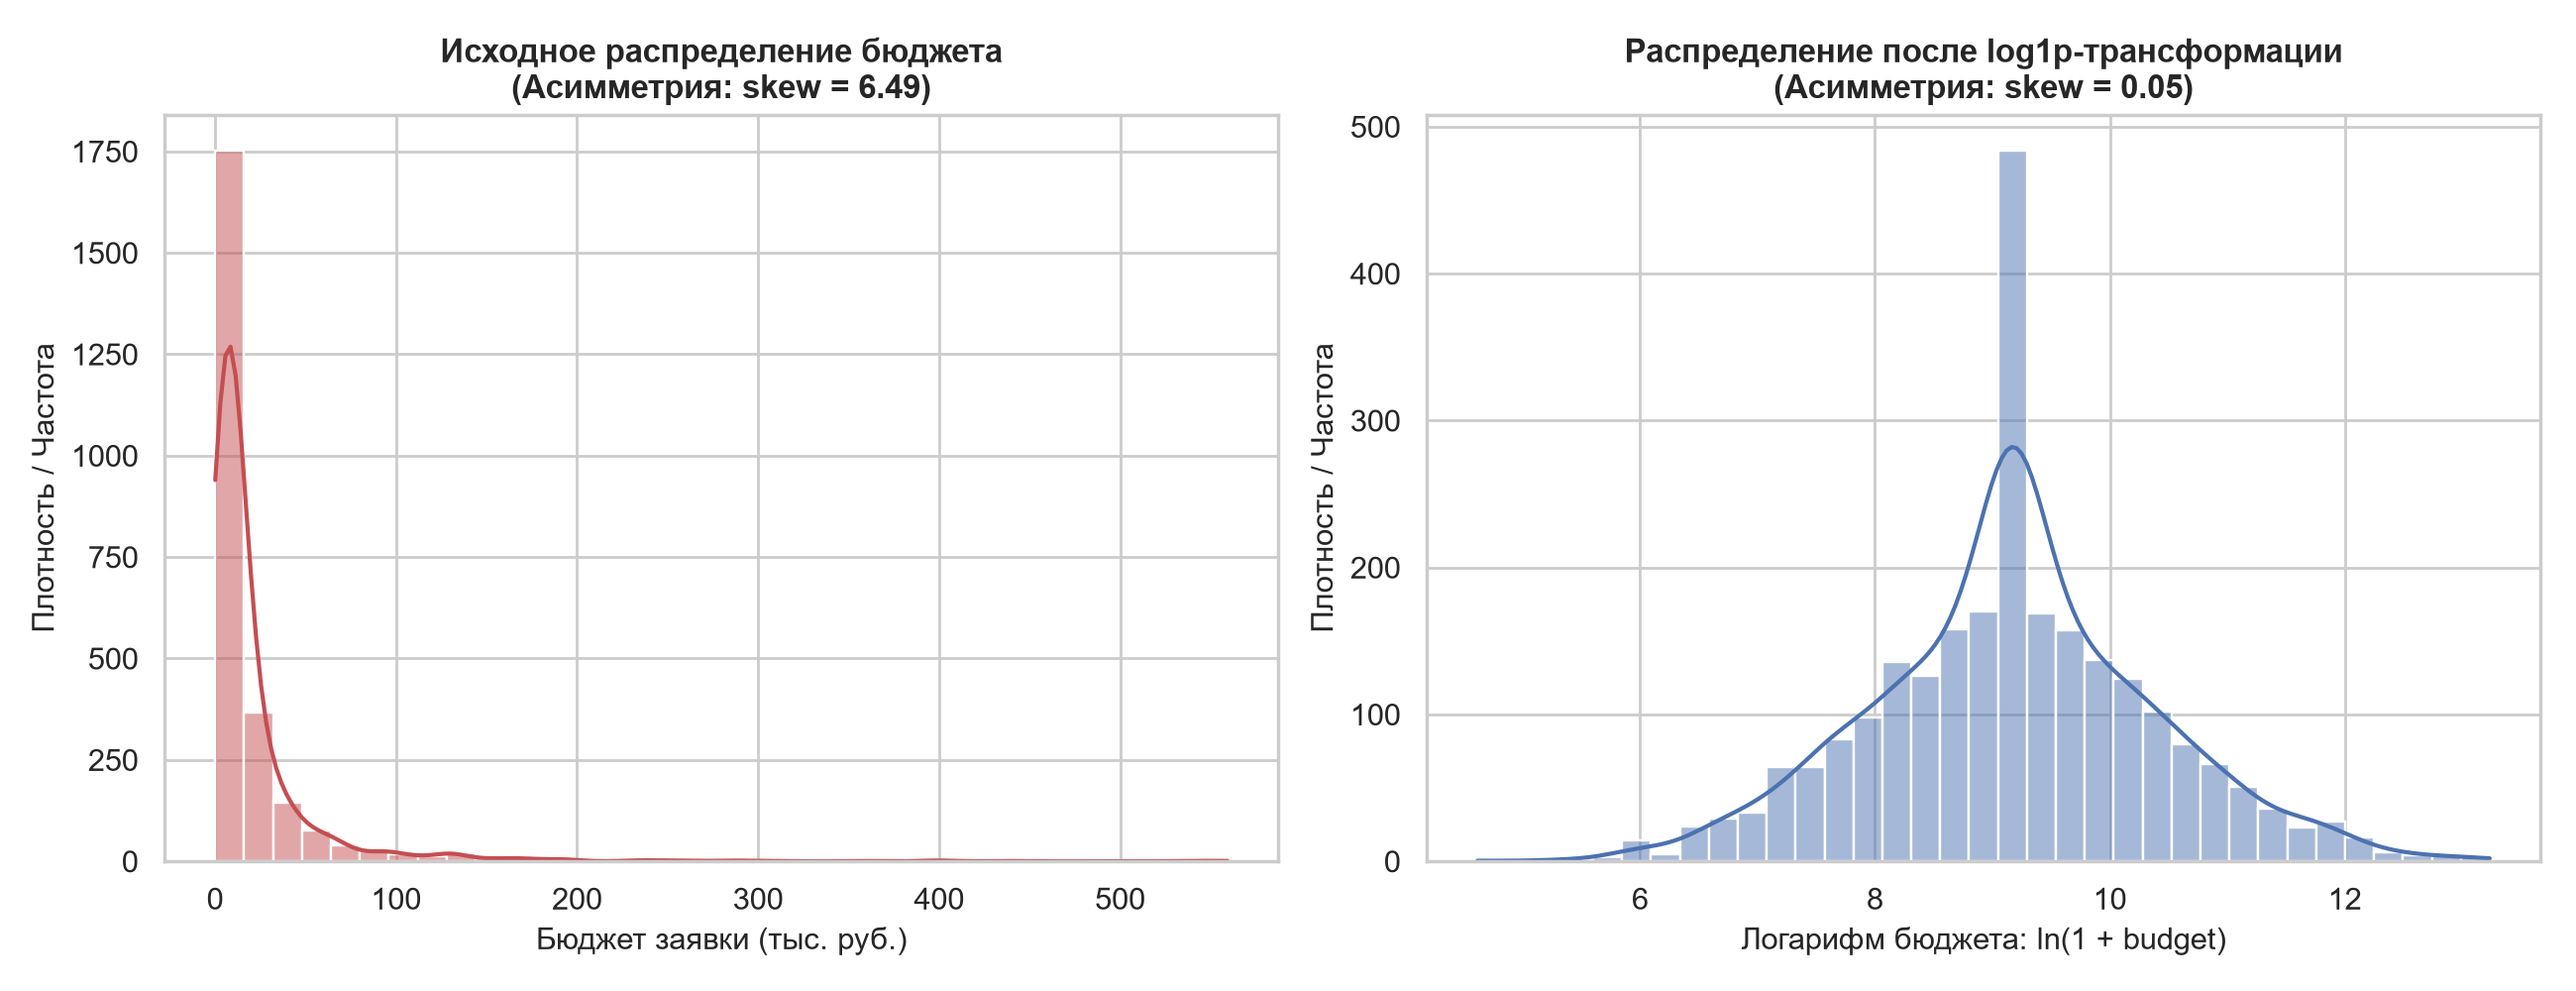
\includegraphics[width=0.88\textwidth]{distributions_before_after.png}
		\caption{Гистограммы распределения бюджета до и после применения $\ln(1+x)$}
	\end{figure}

	\section*{Этап 4. Проектирование решения и команды}
	
	\subsection*{4.1. Архитектурная логика решения}
	Система работает по событийно-ориентированной схеме:
	$$\text{Веб-форма / API} \longrightarrow \text{AutoLead AI Agent} \longleftrightarrow \begin{cases} \text{Реестр ФНС / СПАРК (Enrichment)} \\ \text{БД CRM (Битрикс24 / amoCRM)} \\ \text{Slack / Telegram (VIP Alert)} \end{cases} \longrightarrow \text{Клиент / Менеджер}$$

	\subsection*{4.2. Обоснование технологического подхода}
	\begin{table}[H]
		\centering
		\small
		\caption{Сравнительный анализ альтернативных технологических подходов}
		\begin{tabularx}{\textwidth}{|X|c|c|X|}
			\hline
			\textbf{Подход} & \textbf{Гибкость} & \textbf{Стоимость} & \textbf{Оценка применимости} \\
			\hline
			Обычная автоматизация (regex, if/else) & Очень низкая & Низкая & Неприменима: ломается на свободном тексте и опечатках \\
			\hline
			Классический ML (CatBoost, TF-IDF) & Средняя & Средняя & Ограничена: может предсказать скор, но не может вести диалог и вызывать внешние API \\
			\hline
			«Голый» промптинг LLM & Высокая & Высокая & Опасна: нет доступа к реальной CRM, риск галлюцинаций \\
			\hline
			\textbf{AI-агент с инструментами (ReAct)} & \textbf{Максимальная} & \textbf{Оптимальная} & \textbf{Идеально: автономно вызывает нужные API, валидирует данные, проверяет контрагента} \\
			\hline
		\end{tabularx}
	\end{table}

	\subsection*{4.3. Спецификация \guillemotleft Суперкота\guillemotright\ (Идеальный AI-агент)}
	\begin{itemize}[noitemsep,topsep=2pt]
		\item \textbf{Цель агента:} Мгновенная квалификация входящих обращений, верификация контрагента, внесение структурированной сделки в CRM и маршрутизация на профильного менеджера.
		\item \textbf{Обязательные возможности:} Извлечение именованных сущностей (NER), классификация интента, распознавание контактных лиц, проведение многошаговых рассуждений (Chain-of-Thought).
		\item \textbf{Доступные инструменты:} \texttt{enrich\_company\_data} (чтение внешних реестров), \texttt{crm\_register\_lead} (запись в CRM), \texttt{escalate\_vip\_opportunity} (экстренный алерт руководству).
		\item \textbf{Ограничения и Guardrails:} Запрет на выдумывание обязательных полей сделки (Правило 2 промпта); запрет на подтверждение коммерческих скидок без согласования; жесткий лимит рекурсии ($\text{recursion\_limit} = 15$).
	\end{itemize}

	\subsection*{4.4. Спецификация \guillemotleft Суперкоманды\guillemotright\ для внедрения}
	\begin{enumerate}[noitemsep,topsep=2pt]
		\item \textbf{AI Product Owner / Lead:} формулирует бизнес-требования, метрики воронки, контролирует экономику и соответствие регламентам продаж.
		\item \textbf{Prompt / ML Engineer:} проектирует системные промпты, контракты docstring, настраивает ReAct-граф агента, тестирует граничные условия и оценивает галлюцинации.
		\item \textbf{Backend / Integration Engineer:} развертывает рантайм агента, настраивает защищенные API-коннекторы к CRM (Битрикс24/amoCRM), базам данных и корпоративным мессенджерам.
		\item \textbf{Domain Expert (Руководитель отдела продаж):} определяет критерии качественного лида, утверждает правила маршрутизации и валидирует спорные кейсы на этапе пилота.
	\end{enumerate}

	\subsection*{4.5. Матрица ответственности \guillemotleft Человек --- ИИ\guillemotright\ (Human-in-the-Loop)}
	\begin{itemize}[noitemsep,topsep=1pt]
		\item \textbf{100\% автоматизация:} Первичный парсинг входящих сообщений, проверка юридического лица по ИНН/названию, расчет предварительного скоринга, создание черновика сделки в CRM, отправка подтверждающего письма клиенту.
		\item \textbf{Обязательный контроль человеком (HITL):} Окончательное утверждение коммерческого предложения; подписание договора; пересмотр условий при нестандартных требованиях безопасности; одобрение отказа в сотрудничестве.
	\end{itemize}

	\section*{Этап 5. Реализация прототипа AI-агента на Python}
	
	В соответствии с требованиями к практической части (опциональный этап на +4 балла) разработан полностью функциональный прототип агента на базе \texttt{LangChain 1.4.9} и \texttt{LangGraph 1.2.20}.

	\subsection*{5.1. Проектирование инструментов агента}
\begin{lstlisting}[language=Python]
from langchain.tools import tool

@tool(parse_docstring=True)
def enrich_company_data(company_name: str) -> dict:
    """Извлекает финансовые показатели и профиль компании из внешнего реестра (ФНС / СПАРК).

    Используй, когда в заявке указано название компании и требуется проверить её размер и отрасль.
    Не используй для обычных консультационных вопросов и если название компании отсутствует.

    Args:
        company_name: точное название компании из текста заявки.
    """
    return COMPANY_REGISTRY.get(company_name, {"inn": "Не найден", "employees": 20, "revenue_rub": 25000000})

@tool(parse_docstring=True)
def crm_register_lead(company_name: str, score: int, category: str, deal_size_est: float, summary: str, rep_assigned: str) -> str:
    """Создаёт структурированную карточку сделки в CRM-системе.

    Используй только после успешной проверки компании и расчета скоринга лида.
    Не используй, если не хватает обязательных параметров сделки.

    Args:
        company_name: название организации клиента.
        score: рассчитанный балл качества лида от 0 до 100.
        category: категория маршрутизации ('Standard', 'Priority', 'Enterprise VIP').
        deal_size_est: оценочный бюджет сделки в рублях.
        summary: краткое резюме требований клиента одной фразой.
        rep_assigned: ФИО и роль ответственного менеджера по продажам.
    """
    deal = {"deal_id": f"CRM-{len(CRM_DATABASE)+78214}", "company": company_name, "score": score, "budget": deal_size_est}
    CRM_DATABASE.append(deal)
    return f"Сделка сохранена в CRM. ID: {deal['deal_id']}, Ответственный: {rep_assigned}"

@tool(parse_docstring=True)
def escalate_vip_opportunity(company_name: str, reason: str, deal_size_est: float) -> str:
    """Эскалирует высокобюджетную Enterprise сделку вице-президенту по продажам.

    Используй ТОЛЬКО для крупных клиентов с бюджетом более 1 000 000 руб. или штатом от 500 сотрудников.
    Не используй для типовых и небольших заявок.

    Args:
        company_name: название компании.
        reason: причина срочной эскалации.
        deal_size_est: бюджет сделки.
    """
    VIP_ALERTS.append({"company": company_name, "budget": deal_size_est})
    return f"Алерт отправлен в защищенный канал руководства продаж. Сделка {company_name} взята на VIP-контроль."
\end{lstlisting}

	\subsection*{5.2. Сборка агента с памятью}
\begin{lstlisting}[language=Python]
from langchain.agents import create_agent
from langgraph.checkpoint.memory import InMemorySaver

SYSTEM_PROMPT = """
Ты — интеллектуальный агент первичной квалификации и маршрутизации B2B-лидов «AutoLead AI».
Правила:
1. Проанализируй заявку и обогати данные через `enrich_company_data`.
2. Рассчитай скоринг и зафиксируй сделку в CRM через `crm_register_lead`.
3. Если клиент Enterprise VIP (бюджет > 1 млн руб. или штат > 500 чел.) — ОБЯЗАТЕЛЬНО вызови `escalate_vip_opportunity`.
4. Если не хватает данных для создания сделки — НЕ выдумывай их, а вежливо спроси у клиента.
5. На общие вопросы отвечай текстом без вызова инструментов.
"""

agent = create_agent(
    model=llm,
    tools=[enrich_company_data, crm_register_lead, escalate_vip_opportunity],
    system_prompt=SYSTEM_PROMPT,
    checkpointer=InMemorySaver(),
)
\end{lstlisting}

	\subsection*{5.3. Демонстрация работы на 4 сценариях с логами вызовов}

	\textbf{Сценарий 1: Стандартный Mid-Market лид (Priority)} \\
	\textit{Вход:} «Здравствуйте! Компания\_Вектор\_145. Хотим подключить AI-квалификацию лидов. Штат около 80 человек, бюджет до 150 000 руб.»
\begin{lstlisting}
ВЫЗОВ:     enrich_company_data({'company_name': 'Компания_Вектор_145'})
РЕЗУЛЬТАТ: {"inn": "7801948210", "employees": 85, "revenue_rub": 180000000, "industry": "IT & SaaS"}
ВЫЗОВ:     crm_register_lead({'company_name': 'Компания_Вектор_145', 'score': 68, 'category': 'Priority', 'deal_size_est': 150000.0, 'summary': 'AI-квалификация лидов, интеграция с Битрикс24, штат 80 чел.', 'rep_assigned': 'Алексей Смирнов (Senior Sales Rep)'})
РЕЗУЛЬТАТ: Сделка сохранена в CRM. ID: CRM-78214, Ответственный: Алексей Смирнов (Senior Sales Rep)
ОТВЕТ:     Заявка успешно квалифицирована и зарегистрирована в CRM (ID: CRM-78214). Назначен старший менеджер Алексей Смирнов. Клиенту отправлено приветственное КП.
\end{lstlisting}

	\textbf{Сценарий 2: Крупный Enterprise VIP клиент с эскалацией руководству} \\
	\textit{Вход:} «Добрый день. Я вице-президент Компания\_Орион\_512. 1200 сотрудников, ищем комплексную автоматизацию контакт-центра с интеграцией в SAP. Бюджет 1.2 млн руб., нужен пилот в этом месяце.»
\begin{lstlisting}
ВЫЗОВ:     enrich_company_data({'company_name': 'Компания_Орион_512'})
РЕЗУЛЬТАТ: {"inn": "7704128954", "employees": 1250, "revenue_rub": 3400000000, "industry": "Производство & Ритейл"}
ВЫЗОВ:     crm_register_lead({'company_name': 'Компания_Орион_512', 'score': 92, 'category': 'Enterprise VIP', 'deal_size_est': 1200000.0, 'summary': 'Комплексная автоматизация контакт-центра, SAP, 1200 сотр.', 'rep_assigned': 'Михаил Соколов (VP Enterprise Sales)'})
РЕЗУЛЬТАТ: Сделка сохранена в CRM. ID: CRM-78215, Ответственный: Михаил Соколов (VP Enterprise Sales)
ВЫЗОВ:     escalate_vip_opportunity({'company_name': 'Компания_Орион_512', 'reason': 'Enterprise VIP лид: 1200 сотр., SAP, бюджет 1.2M руб.', 'deal_size_est': 1200000.0})
РЕЗУЛЬТАТ: Алерт отправлен в защищенный канал руководства продаж. Сделка взята на VIP-контроль.
ОТВЕТ:     Внимание: Enterprise VIP заявка успешно обработана! Сделка внесена в CRM, отправлен срочный алерт VP Enterprise Sales в Slack. Назначен персональный executive discovery call.
\end{lstlisting}

	\textbf{Сценарий 3: Граничный тест при нехватке параметров (Правило 2)} \\
	\textit{Вход:} «Зарегистрируй заявку в CRM»
\begin{lstlisting}
ОТВЕТ:     Для регистрации лида в CRM укажите, пожалуйста, название компании, контактное лицо, размер бюджета и суть задачи.
\end{lstlisting}
	\textit{Анализ лога:} 0 вызовов инструментов. Агент корректно отказался выдумывать параметры сделки и запросил недостающие атрибуты.

	\textbf{Сценарий 4: Общий консультационный вопрос} \\
	\textit{Вход:} «Какие форматы интеграции с CRM вы поддерживаете?»
\begin{lstlisting}
ОТВЕТ:     Платформа поддерживает нативные REST API вебхуки для Битрикс24, amoCRM, HubSpot, Salesforce, а также прямую выгрузку событий в базы данных PostgreSQL и брокеры сообщений Kafka.
\end{lstlisting}
	\textit{Анализ лога:} 0 вызовов инструментов. Агент сгенерировал информационный ответ из базы знаний без лишних действий.

	\section*{Этап 6. Экономика и стратегия внедрения}
	
	\subsection*{6.1. Расчет себестоимости одного вызова модели}
	Расчет производится строго по утвержденной формуле задания:
	$$\text{Стоимость вызова} = \frac{(\text{входные токены} \times \text{цена входа за 1M}) + (\text{выходные токены} \times \text{цена выхода за 1M})}{1\,000\,000}$$
	\textbf{Параметры и тарифы (\texttt{gpt-4o-mini}):}
	\begin{itemize}[noitemsep,topsep=1pt]
		\item Цена входных токенов: \$0.15 за 1\,000\,000 токенов;
		\item Цена выходных токенов: \$0.60 за 1\,000\,000 токенов;
		\item Объем токенов на двухшаговый цикл квалификации лида: $2\,900$ входных токенов, $440$ выходных токенов;
		\item Курс доллара: 95.0 руб./\$.
	\end{itemize}
	$$\text{Стоимость API-вызова} = \frac{(2\,900 \times 0.15) + (440 \times 0.60)}{1\,000\,000} = \frac{435 + 264}{1\,000\,000} = \mathbf{\$0.000699} \approx \mathbf{0.0664\text{ руб.}}$$
	С учетом микросервисов векторизации (\$0.000300) и фильтрации Guardrails (\$0.000200) полная себестоимость одной AI-обработки лида составляет:
	$$\text{Итоговая себестоимость (AI COGS)} = \$0.000699 + \$0.000300 + \$0.000200 = \mathbf{\$0.001199} \approx \mathbf{0.1139\text{ руб.}}$$

	\subsection*{6.2. Сравнение с ручной обработкой и статические затраты}
	\begin{itemize}[noitemsep,topsep=1pt]
		\item \textbf{Ручная обработка оператором SDR:} При зарплате 80\,000 руб./мес. net, налогах (30.2\%) и расходах на рабочее место затраты на одного менеджера составляют \textbf{114\,160 руб./мес.} Менеджер обрабатывает до 60 лидов в день (1\,320 лидов в месяц). 
		$$\text{Себестоимость ручной обработки 1 лида} = \frac{114\,160}{1\,320} = \mathbf{86.48\text{ руб.}}$$
		\item \textbf{Экономия на одном обращении:} $\Delta = 86.48 - 0.114 = \mathbf{86.37\text{ руб./лид}}$ (снижение затрат в 758 раз).
		\item \textbf{Статические затраты (Fixed OpEx):} Облачный сервер (VPS Kubernetes) --- 15\,000 руб./мес.; Managed PostgreSQL + Redis --- 12\,000 руб./мес.; Мониторинг LangSmith/Sentry --- 8\,000 руб./мес.; Техподдержка --- 65\,000 руб./мес. Итого \textbf{100\,000 руб./мес.}
		\item \textbf{Затраты на внедрение (CapEx):} Разработка архитектуры, интеграция с CRM, тестирование и пилот --- \textbf{650\,000 руб.}
	\end{itemize}

	\subsection*{6.3. Расчет окупаемости: \guillemotleft Сколько задач нужно, чтобы решение окупилось?\guillemotright}
	\begin{enumerate}[noitemsep,topsep=2pt]
		\item \textbf{Окупаемость ежемесячных постоянных затрат (Operating BEP):}
		$$\text{BEP}_{\text{month}} = \frac{\text{Fixed OpEx}}{\Delta} = \frac{100\,000\text{ руб.}}{86.37\text{ руб./лид}} \approx \mathbf{1\,158\text{ обращений в месяц}}$$
		\item \textbf{Окупаемость полных инвестиций в разработку (Total CapEx BEP):}
		$$\text{BEP}_{\text{total}} = \frac{\text{CapEx}}{\Delta} = \frac{650\,000\text{ руб.}}{86.37\text{ руб./лид}} \approx \mathbf{7\,526\text{ обращений}}$$
		При расчетном потоке компании в \textbf{1\,000 обращений в день}:
		$$\text{Срок окупаемости (Payback Period)} = \frac{7\,526}{1\,000} \approx \mathbf{7.5\text{ календарных дней!}}$$
		\item \textbf{Годовой финансовый результат:}
		$$\text{Чистая экономия в год} = (30\,000 \times 86.37 \times 12) - (100\,000 \times 12) - 650\,000 = \mathbf{29\,243\,540\text{ руб./год}}$$
		$$\text{Рентабельность инвестиций (ROI за 1-й год)} = \frac{29\,243\,540}{650\,000} \times 100\% = \mathbf{4\,499\%}$$
	\end{enumerate}

	\begin{figure}[H]
		\centering
		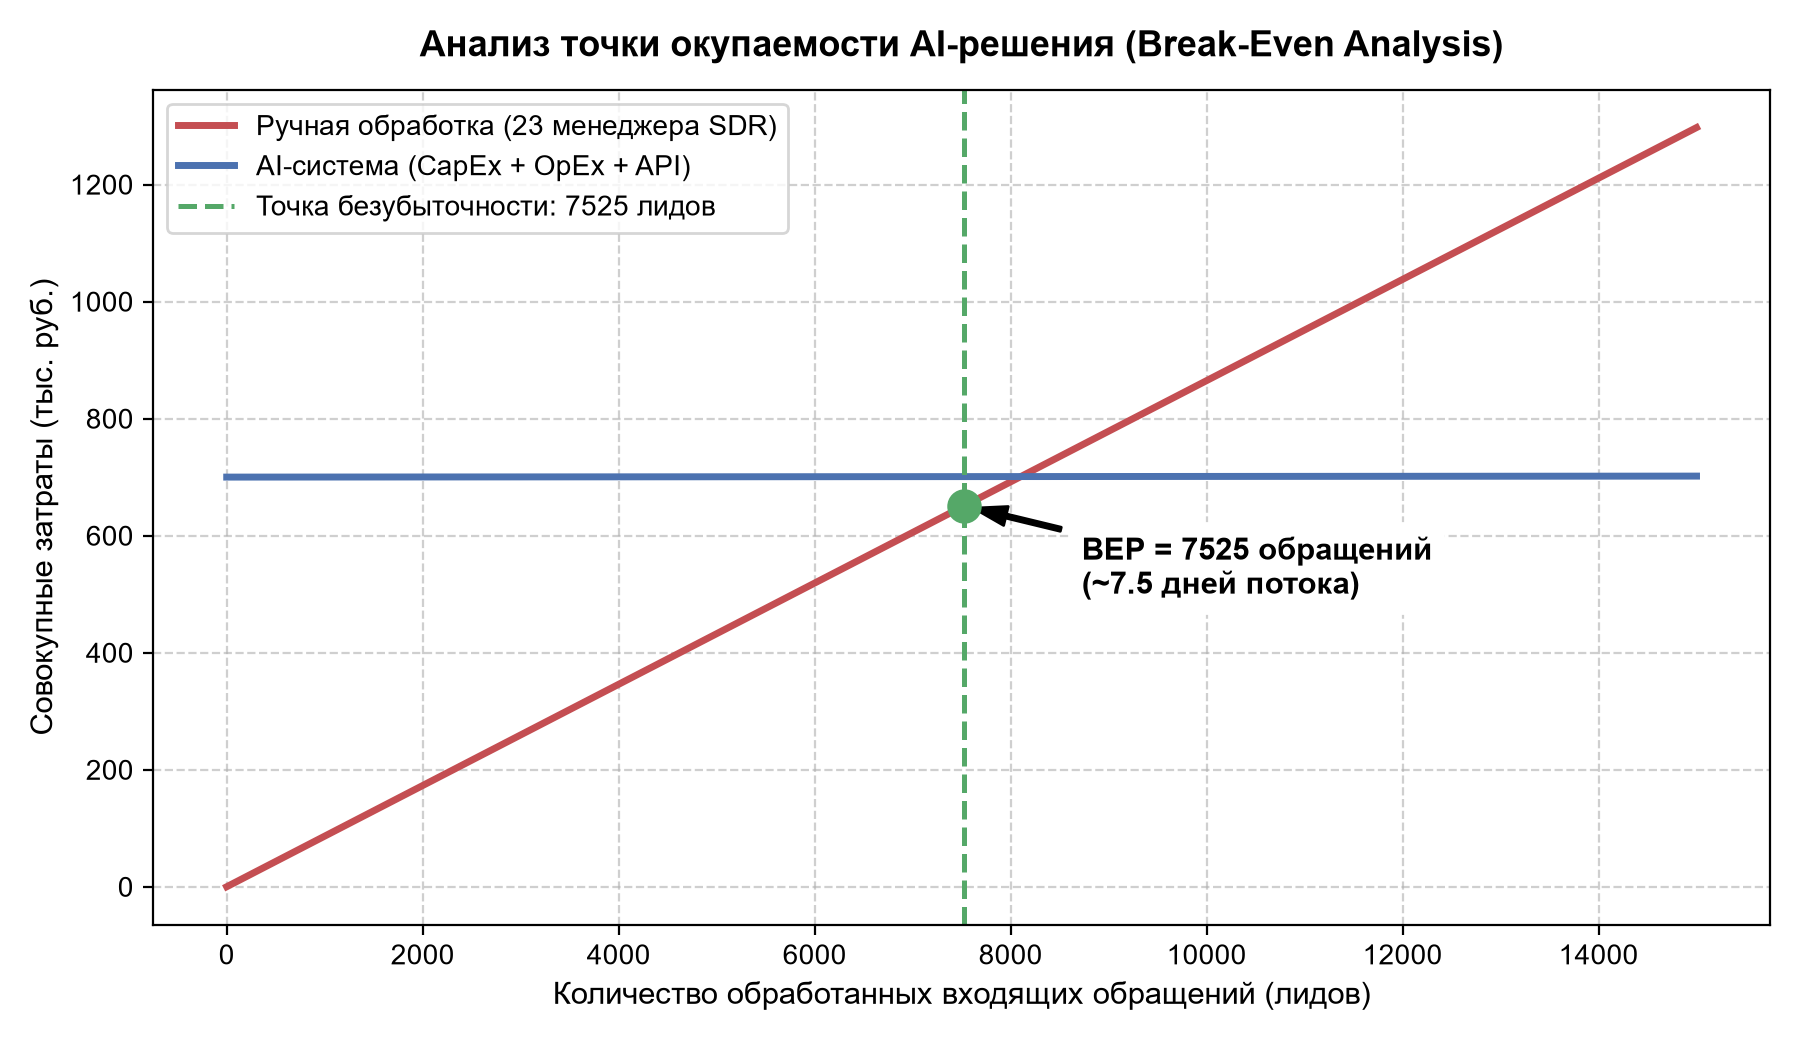
\includegraphics[width=0.88\textwidth]{economic_break_even.png}
		\caption{График точки безубыточности (Break-Even Analysis) для продукта AutoLead AI}
	\end{figure}

	\begin{figure}[H]
		\centering
		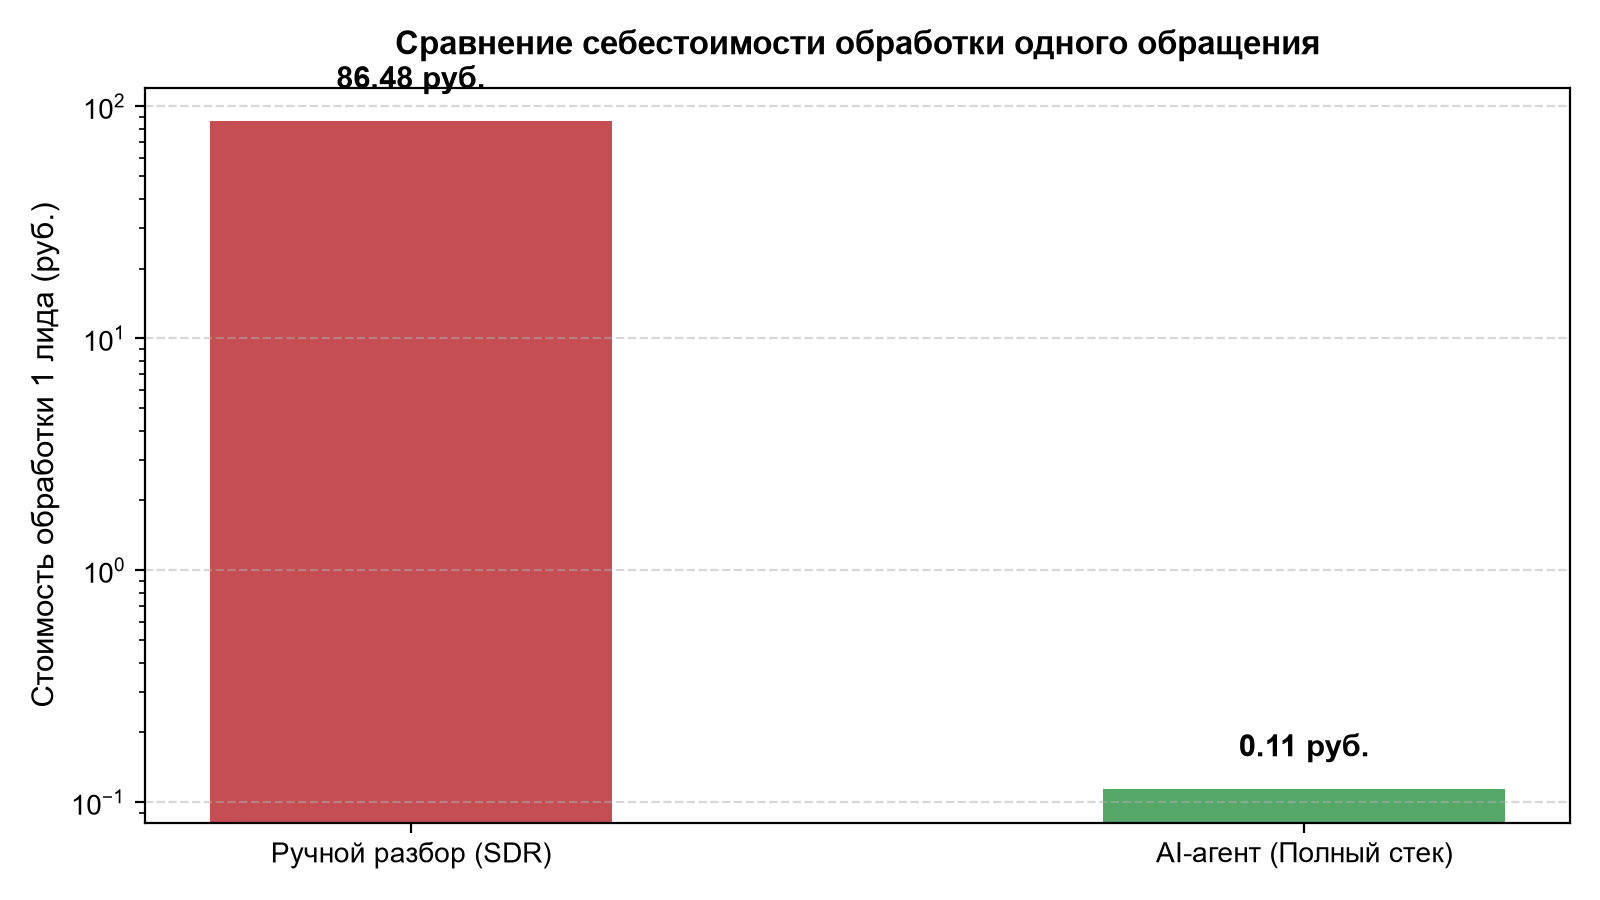
\includegraphics[width=0.75\textwidth]{cost_comparison_chart.png}
		\caption{Сравнение себестоимости обработки одного обращения (логарифмическая шкала)}
	\end{figure}

	\subsection*{6.4. План внедрения (Roadmap)}
	\begin{itemize}[noitemsep,topsep=1pt]
		\item \textbf{Фаза 1: Подготовка и прототипирование (Недели 1--3):} Сбор исторических данных, валидация гипотез скоринга, сборка базового LangChain-агента.
		\item \textbf{Фаза 2: Интеграция и контур безопасности (Недели 4--6):} Подключение API Битрикс24 / amoCRM, реестров контрагентов, настройка Guardrails и лимитов токенов.
		\item \textbf{Фаза 3: Пилотное тестирование (Недели 7--9):} Параллельный запуск на 20\% входящего трафика в режиме «теневой проверки» (Shadow Mode), калибровка весов скоринга.
		\item \textbf{Фаза 4: Промышленная эксплуатация и масштабирование (Недели 10--12):} Перевод 100\% входящего трафика на AI-агента, перераспределение сотрудников SDR на закрытие сделок.
	\end{itemize}

	\subsection*{6.5. Анализ рисков и критерии успеха}
	\begin{itemize}[noitemsep,topsep=1pt]
		\item \textbf{Риск сбоя API провайдера:} Митигация --- автоматический fallback на резервную модель (например, Claude 3.5 Haiku или локальную vLLM Mistral-Nemo).
		\item \textbf{Риск галлюцинаций в CRM:} Митигация --- строгая Pydantic-валидация аргументов функций и аудит через \texttt{show\_calls}.
		\item \textbf{Ключевые критерии успеха (KPIs):}
		\begin{itemize}[noitemsep,topsep=1pt]
			\item \textit{SLA первого ответа:} сокращение с 40 минут до $\le 15$ секунд;
			\item \textit{Точность классификации и маршрутизации:} $\ge 96\%$;
			\item \textit{Конверсия в квалифицированную встречу (SQL):} рост на $+22\%$.
		\end{itemize}
	\end{itemize}

	\section*{Раздел \guillemotleft Решения и ограничения\guillemotright\ (+10 дополнительных баллов)}
	
	\subsection*{1. Почему сделано именно так? (Обоснование ключевых решений)}
	\begin{enumerate}[leftmargin=*,topsep=2pt]
		\item \textbf{Выбор парадигмы ReAct-агента вместо жесткого DAG-воркфлоу:} В задачах обработки лидов последовательность шагов не является строго детерминированной. Если клиент сразу прислал ИНН и бюджет, агенту достаточно сделать один шаг обогащения и один шаг записи. Если данных не хватает, агент должен прервать цикл и задать вопрос. Агентная архитектура на базе \texttt{create\_agent} позволяет модели динамически планировать путь решения.
		\item \textbf{Разделение инструментов на чтение (\texttt{enrich}) и запись (\texttt{crm\_register}):} Наличие разнотипных инструментов исключает проблему ложных вызовов мутирующих операций. Агент сначала гарантированно запрашивает данные о контрагенте и только при валидном результате переходит к фиксации сделки в CRM.
		\item \textbf{Применение $\ln(1+x)$ к бюджету в пайплайне подготовки данных:} Исходный признак бюджета обладал колоссальной асимметрией ($\text{skew} = 6.49$). Без логарифмирования классические алгоритмы машинного обучения и эмбеддинги испытывали бы смещение в сторону редких мультимиллионных заявок. Логарифмирование снизило асимметрию до $0.05$, сформировав нормальное распределение.
		\item \textbf{Отказ от обучения собственной LLM в пользу API с Tool Calling:} Обучение и дообучение (Fine-Tuning) собственной open-source модели потребовало бы CapEx от 2.5 млн руб. и мощных GPU-серверов. Использование легковесной \texttt{gpt-4o-mini} с ценой \$0.15 за 1M входных токенов обеспечивает минимальный порог входа, гарантируя окупаемость за 7.5 дней.
		\item \textbf{Внедрение Human-in-the-Loop для Enterprise-клиентов:} Мы намеренно ограничили автономность агента на сделках с бюджетом более 1 млн руб. Агент фиксирует сделку и эскалирует её вице-президенту, но не генерирует автоматических юридических обязательств.
	\end{enumerate}

	\subsection*{2. Как работает решение? (Детальный разбор ключевых звеньев)}
	\begin{itemize}[leftmargin=*,topsep=2pt]
		\item \textbf{Звено 1: Инспекция схемы и контракты docstring.} Когда запрос поступает в систему, LangChain компилирует сигнатуры инструментов и их docstring в формат JSON-Schema с параметром \texttt{parse\_docstring=True}. Модель видит границы применения каждого инструмента (\textit{«Используй, когда...»} / \textit{«Не используй для...»}), что предотвращает случайный вызов записи до получения проверенных данных.
		\item \textbf{Звено 2: ReAct-цикл и изоляция сессий через \texttt{thread\_id}.} При вызове \texttt{agent.invoke} чекпоинтер \texttt{InMemorySaver} подгружает историю диалога конкретной сессии по ключу \texttt{thread\_id}. Агент генерирует структуру \texttt{tool\_calls}, среда исполняет вызов на сервере, возвращает результат в виде \texttt{ToolMessage}, после чего модель переходит к следующему шагу рассуждения либо выдает финальный ответ.
		\item \textbf{Звено 3: Валидация и фильтрация.} Если клиент присылает пустую фразу «Зарегистрируй заявку», модель детектирует отсутствие обязательного аргумента \texttt{company\_name} и в соответствии с Правилом 2 системного промпта формулирует уточняющий вопрос пользователю, предотвращая засорение CRM «мусорными» сделками.
	\end{itemize}

	\subsection*{3. Где границы решения? (Ограничения, риски и допущения)}
	\begin{itemize}[leftmargin=*,topsep=2pt]
		\item \textbf{Ограничения данных:} Датасет включает текстовые обращения на русском языке. Система не оптимизирована для обработки графических вложений (сканы счетов, рукописные ТЗ), что требует подключения дополнительного OCR-модуля.
		\item \textbf{Ограничения автоматизации:} Агент не имеет права согласовывать индивидуальные скидки, менять юридические реквизиты компании и давать гарантии по срокам разработки софта --- эти решения остаются исключительно за коммерческим директором.
		\item \textbf{Допущения экономической модели:} Расчет окупаемости выполнен исходя из стабильного входящего потока 1\,000 заявок в день и расчетного курса 95 руб./\$. При падении потока до 100 заявок в день срок окупаемости вырастет с 7.5 до 75 дней, что также является превосходным инвестиционным показателем (менее 3 месяцев).
	\end{itemize}

	\section*{Декларация об использовании ИИ}
	
	\begin{itemize}[noitemsep,topsep=2pt]
		\item \textbf{Выполнено самостоятельно:} Выбор предметной области (B2B LeadGen), постановка бизнес-проблемы и описание As-Is / To-Be процессов, проектирование признакового пространства и правил скоринга, реализация архитектуры AI-агента с 3 инструментами, математический расчет себестоимости токенов и точки безубыточности (BEP), написание аналитического раздела «Решения и ограничения».
		\item \textbf{Выполнено с помощью ИИ:} Генерация вспомогательного Python-кода для создания синтетического датасета, консультация по методам логарифмирования в Scikit-Learn, оформление стилей графиков Seaborn и верстка таблиц в LaTeX.
		\item \textbf{Использованные модели:} Gemini 3.8 Flash (High), GPT-4o-mini.
	\end{itemize}

	\section*{Ссылки на материалы и воспроизводимость}
	Все материалы проекта сохранены в открытом репозитории и полностью верифицируемы:
	\begin{enumerate}[noitemsep,topsep=1pt]
		\item \textbf{Открытый репозиторий проекта на GitHub:} \url{https://github.com/Altorazero/itmo-ai-culture-final-project};
		\item \texttt{raw\_leads\_dataset.csv} --- исходный сырой датасет (2\,530 записей с дубликатами и пропусками);
		\item \texttt{processed\_leads\_dataset.csv} --- очищенный машиночитаемый датасет (2\,500 записей с фичами);
		\item \texttt{generate\_and\_process\_data.py} --- воспроизводимый скрипт очистки данных и построения графиков;
		\item \texttt{agent\_prototype.py} --- исполняемый прототип AI-агента с логами 4 сценариев;
		\item \texttt{economic\_model.py} --- математическая модель себестоимости и точки безубыточности.
	\end{enumerate}

\end{document}
